\chapter{Implementación}
{\color{blue}



La implementación de la aplicación se realiza con \textbf{Kaa IoT} tal y como se analizo anteriormente \ref{eleccion-framework}. Para empezar a usar el framework, hay que registrarse en sistema. Una vez registrados tendremos acceso a nuestro \textit{dashboard} \footnote{Hace referencia al cuadro de mandos al que tenemos acceso para interactuar con nuestro dispositivo y todas las posibles configuraciones}. En este capítulo se trata de mostrar una guía con la que se consiga conectar un dispositivo, recoger y enviar datos desde/hacia el dispositivo y mostrar las opciones que nos ofrece Kaa IoT como framework IoT. Para empezar, vamos a conectar nuestro primer dispositivo.

\begin{figure}[hb!]
    \centering
    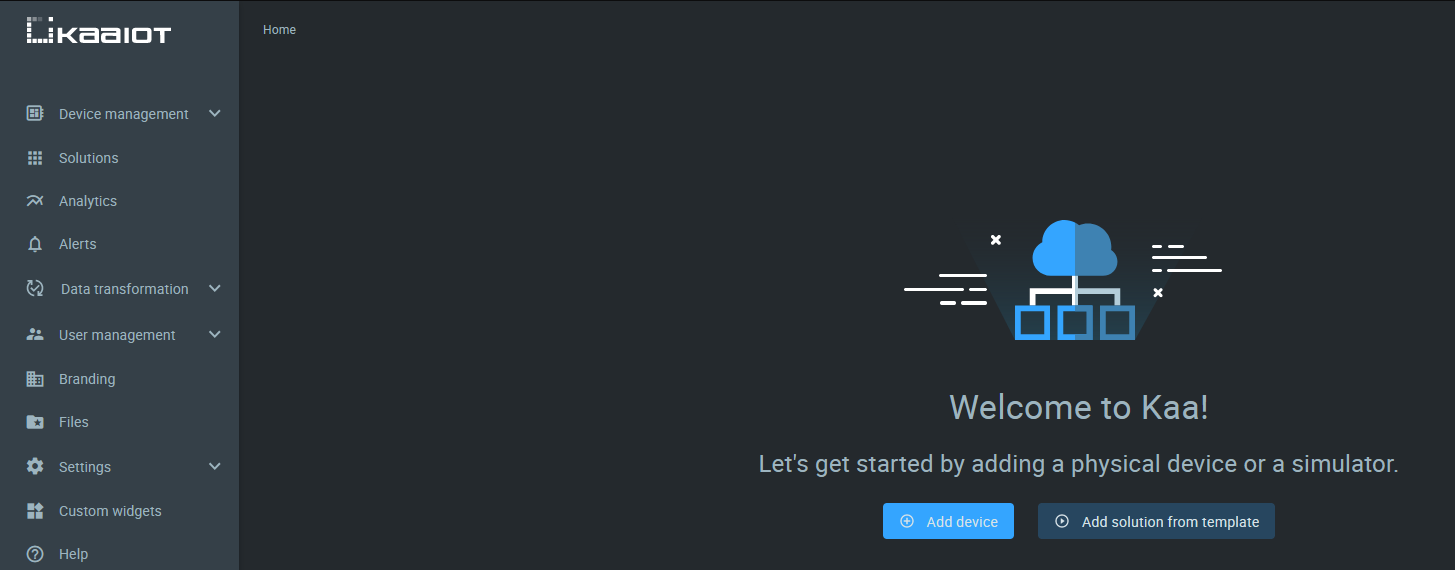
\includegraphics[width=\linewidth]{imagenes/dashboard.png}
    \caption{Dashboard Kaa IoT.}
    \label{fig:figure5}
\end{figure}


\section{Conectar dispositivo}

En este apartado se trata de explicar el proceso de conexión de un dispositivo con nuestra aplicación, desde crear un endpoint hasta ver la información del dispositivo en nuestra interfaz de usuario. Esto engloba varios términos y conceptos que se van a definir a continuación. \cite{kaaiotConnectDevice}

\subsection{Términos y conceptos} \label{initial-terms}

\subsubsection{Endpoints}

Los endpoints representan ``el elemento de las cosas`` del IoT. Un endpoint es cualquier dispositivo terminal que se quiera gestionar, en nuestro caso desde Kaa IoT. Un endpoint puede ser un dispositivo físico o una emulación de software del mismo. Todos los datos que llegan a la aplicación están asociados a endpoints. \cite{kaaiotConcepts}

Para ser precisos, un endpoint puede ser una unidad menor que un dispositivo, lo que significa que un dispositivo físico puede incluir múltiples endpoints. Por ejemplo, quieres gestionar un termostato, para que el aire acondicionado se encienda y apague automáticamente a cierta temperatura.

Se puede gestionar el termostato de una de las siguientes maneras:

\begin{itemize}
    \item Toda la unidad del termostato actúa como un endpoint único que intercambia datos con el servidor.
    \item Los componentes del termostato, como los sensores de temperatura y humedad, interruptor de encendido/apagado, actúan como endpoints individuales.
\end{itemize}

\subsubsection{ID de Endpoint}

El ID de endpoints se utiliza para identificar de forma única un endpoint dentro de una instancia. Un ID de endpoints suele ser un UUID generado automáticamente por el framework en el momento de crear un nuevo endpoint. No obstante, también se permiten los ID de endpoints definidos por el usuario. El ID de los endpoints no puede modificarse una vez creado.

Todos los datos de los endpoints, como los atributos de los metadatos, los puntos de datos de series temporales recopilados, los comandos, etc., están asociados a un ID de endpoint específico. Siempre que recupere o gestione datos relacionados con endpoints en Kaa, principalmente a través de la API REST, se verá los ID de endpoints.

\subsubsection{Token del Endpoint} \label{llamada-mqtt}

Los tokens de endpoints se utilizan para la identificación de endpoints cuando se intercambian datos relacionados con los endpoints, utilizando los protocolos compatibles basados en MQTT y HTTP. Los tokens de endpoint son únicos dentro de una aplicación IoT y se asignan exactamente a un endpoint.

Cuando llega un mensaje de un cliente, el token del endpoint se resuelve en el correspondiente ID del endpoint. Un ejemplo sobre el protocolo MQTT, el token del endpoint va dentro de la llamada MQTT, por ejemplo:

\begin{lstlisting}[language=HTML]
kp1/<APPLICATION_VERSION>/epmx/<ENDPOINT_TOKEN>/get
\end{lstlisting}

Normalmente, los tokens son cadenas generadas automáticamente por el framework, pero también se puede crear un token como el usuario quiera, por ejemplo, por el número de serie del dispositivo, dirección MAC, etc.

\subsubsection{Metadatos del endpoint}

Los metadatos de los endpoints son un conjunto de atributos clave-valor asociados a un endpoint. Se representan en el framework como un documento JSON de formato arbitrario.

Los metadatos de endpoints suelen incluir alguna información relacionada con los endpoints, como la ubicación, la descripción, el número de serie, la versión de hardware, etc. Los metadatos se almacenan en el servicio de registro de endpoints y pueden leerse o actualizarse de dos maneras:

\begin{itemize}
    \item A través de la capa de comunicación.
    \item A través de la API REST.
\end{itemize}

También se pueden gestionar los metadatos mediante la interfaz de usuario del framework.

\subsubsection{Aplicaciones y versiones}

Las aplicaciones en Kaa IoT sirven como contenedores para endpoints de diferentes tipos. Se puede tener una aplicación que contenga todos los endpoints que representan a un determinado dispositivo, y una aplicación para otro dispositivo, independiente de la otra aplicación. Las aplicaciones IoT también albergan toda la configuración del sistema necesaria para que el framework conozca las capacidades de sus dispositivos conectados y cómo trabajar con ellos.

Puede pasar que ya hemos configurado nuestro dispositivo, pero queremos implementar una nueva característica. Al implementarla se actualiza el firmware del dispositivo y se empieza a desplegar pero, ¿como diferenciamos entre los dispositivos que ya tienen el nuevo firmware y las que no? Aquí aparecen las versiones de una aplicación.

Cada aplicación puede tener varias versiones al mismo tiempo. Cada versión representa un conjunto de capacidades soportadas por los endpoints. En cualquier momento, cada endpoint está asociado a una versión de su aplicación. El conocimiento de la versión actual de la aplicación de un endpoint ayuda al framework a entender qué funcionalidad soporta el endpoint, cómo se formatean los datos, etc. Se puede utilizar las versiones para hacer evolucionar los dispositivos añadiendo o retirando funcionalidades mientras mantiene sus versiones antiguas en funcionamiento. Para diferenciar llamadas entre versiones se puede indicar como hemos visto en \ref{llamada-mqtt}.

\subsection{Pasos a seguir}

\subsubsection{Crear una aplicación y una versión}

Como hemos visto en \ref{initial-terms}, para registrar un endpoint en nuestro framework necesitamos una aplicación y una versión de esta. Esto podemos gestionarlo desde la interfaz de usuario, concretamente en la sección ``Applications``, una vez en la sección usaremos el botón de ``Add application``. Introduciremos el nombre de la aplicación (campo obligatorio) y tendremos la posibilidad de introducir una descripción. En nuestro caso la aplicación se llamará ``TFG-DASIoT``. \\

Hay que tener en cuenta que tanto las aplicaciones como las versiones tienen:

\begin{itemize}
    \item Nombres autoasignados e inmutables que suelen ser como  \textbf{7bfdd6b9-ff44-4098-a4dc-58c0f3c9f693-v1}. Se utilizarán para las llamadas a la API, la integración con el cliente, etc.
    \item Nombres de visualización arbitrarios que se pueden cambiar en cualquier momento. Estos nombres se utilizan en la interfaz de usuario de la plataforma para una mejor experiencia de usuario. Por ejemplo, en nuestro caso el nombre de la aplicación y la descripción que hayamos puesto.
\end{itemize}

\begin{figure}[hb!]
    \centering
    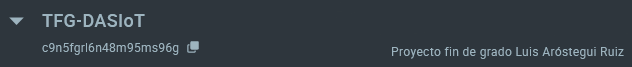
\includegraphics[width=\linewidth]{imagenes/app-creada.png}
    \caption{Nombre y descripción de la aplicación}
    \label{fig:figure6}
\end{figure}

En la imagen también se puede observar como hay un identificador justo debajo del nombre que le hemos asignado a la aplicación, esto es para referenciar de manera univoca a esta. Y ahora que tenemos la aplicación, creamos una versión de esta.

\begin{figure}[ht!]
    \centering
    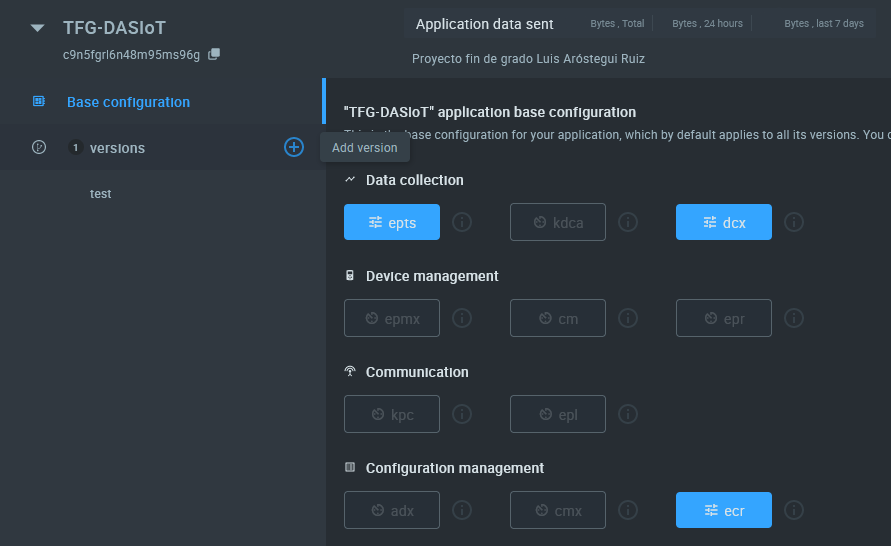
\includegraphics[width=\linewidth]{imagenes/app-version.png}
    \caption{Versiones de la aplicación}
    \label{fig:figure7}
\end{figure}

La primera versión que hemos creado se llama ``test``. Y en la información de la aplicación podemos ver los servicios que tenemos activos.

\begin{itemize}
    \item \textbf{Data collection}. \textit{epts}, se refiere al servicio de series temporales de endpoints. Recibe muestras de datos de endpoints y los transforma en series temporales. \textit{dcx}, es un servicio de recogida de datos, permite a los endpoints enviar muestras de datos de telemetría a la aplicación.
    \item \textbf{Configuration management}. \textit{ecr}, configuración del repositorio del endpoint, almacena los datos de configuración de los endpoints y proporciona una API REST para la gestión.
\end{itemize}

\subsubsection{Crear un endpoint}

En la sección de ``Devices`` de nuestro dashboard, podremos añadir un nuevo dispositivo. Aqui indicaremos, la aplicación a la que va a estar asociada el dispositivo, un nombre para nuestro endpoint y opcionalmente podremos añadir metadatos.

\begin{figure}[p]
    \centering
    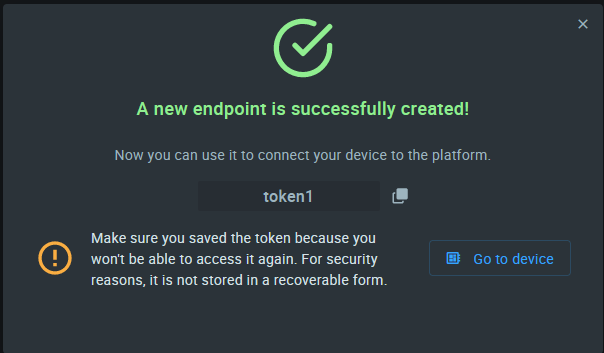
\includegraphics[width=\linewidth]{imagenes/device-added.png}
    \caption{Endpoint creado}
    \label{fig:figure8}
\end{figure}

\begin{figure}[p]
    \centering
    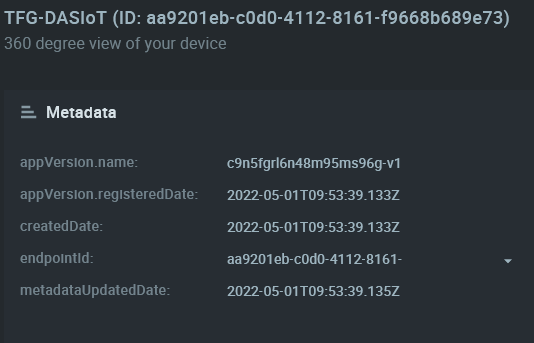
\includegraphics[width=\linewidth]{imagenes/device-created-view.png}
    \caption{Datos del dispositivo creado}
    \label{fig:figure9}
\end{figure}

En nuestro caso, para referirnos al endpoint lo hacemos mediante el \textit{token endpoint} \ref{llamada-mqtt}, que como vemos en \ref{fig:figure8}, se llama token1. Esto lo usaremos en nuestra llamada mqtt para hacer referencia a este dispositivo.\\

Para ver todos los datos del dispositivo se nos muestra como vemos en \ref{fig:figure9}. Donde podemos ver la aplicación a la que esta asociada, la fecha de creación y de su última actualización.

\newpage

\subsubsection{Conectar un cliente}

Una vez ya hemos creado nuestro primer endpoint, podemos conectar un cliente y obtener y enviar algunos metadatos. Como se analizó \ref{eleccion-framework}, Kaa IoT es un framework que soporta varios protocolos donde nos encontramos con HTTP y MQTT \ref{protocolos}.

Para hacer uso de los protocolos y completar la integración del cliente necesitaremos el nombre de la versión y el token del endpoint. En esta sección se va a mostrar como hacer uso de ambos protocolos, concretamente de las órdenes para poder ejecutar la conexión con nuestro dispositivo, en la sección de \textit{Pruebas} \ref{pruebas} se mostrarán los datos que obtenemos tras su ejecución.\\

\paragraph{Conexión mediante HTTP} \label{http-connection} \hspace{0pt} \\

Para obtener todos los atributos de los metadatos con \textbf{HTTP} vamos a hacer uso de cURL \footnote{Es un proyecto de software consistente en una biblioteca y un intérprete de comandos orientado a la transferencia de archivos. Soporta los protocolos FTP, FTPS, HTTP, HTTPS, TFTP, SCP, SFTP, Telnet, DICT, FILE y LDAP, entre otros.} para enviar una solicitud de actualización de datos del dispositivo.

\begin{lstlisting}[language=bash]
curl - -location - -request POST 'https://connect.cloud.kaaiot.com:443/kp1/
<app-version-name>/epmx/<endpoint-token>/update/keys' \
- -data-raw '{
    "model": "BFG 9000",
    "mac": "00-14-22-01-23-45"
}'
\end{lstlisting}

Ejecutando esta instrucción añadiremos nuevos metadatos a nuestro dispositivo, concretamente la dirección física y el modelo de este.

\paragraph{Conexión mediante MQTT} \label{mqtt-connection} \hspace{0pt} \\

Para hacer la conexión mediante \textbf{MQTT} se ha optado por la opción de usar Python en su versión 3.10, obtenemos un código como el siguiente.

\begin{lstlisting}[language=Python]
import itertools
import json
import queue
import random
import string
import sys
import time

import paho.mqtt.client as mqtt
from decouple import config

KPC_HOST = config('KPC_HOST', cast=str)
KPC_PORT = config('KPC_PORT', cast=int)

APPLICATION_VERSION = config('APPLICATION_VERSION', cast=str)
ENDPOINT_TOKEN = config('ENDPOINT_TOKEN', cast=str)


class MetadataClient:

    def __init__(self, client):
        self.client = client
        self.metadata_by_request_id = {}
        self.global_request_id = itertools.count()
        get_metadata_subscribe_topic = f'kp1/{APPLICATION_VERSION}/epmx/{ENDPOINT_TOKEN}/get/#'
        self.client.message_callback_add(get_metadata_subscribe_topic, self.handle_metadata)

    def handle_metadata(self, client, userdata, message):
        request_id = int(message.topic.split('/')[-2])
        if message.topic.split('/')[-1] == 'status' and request_id in self.metadata_by_request_id:
            print(f'<--- Received metadata response on topic {message.topic}')
            metadata_queue = self.metadata_by_request_id[request_id]
            metadata_queue.put_nowait(message.payload)
        else:
            print(
                f'<--- Received bad metadata response on topic {message.topic}:\n{str(message.payload.decode("utf-8"))}')

    def get_metadata(self):
        request_id = next(self.global_request_id)
        get_metadata_publish_topic = f'kp1/{APPLICATION_VERSION}/epmx/{ENDPOINT_TOKEN}/get/{request_id}'

        metadata_queue = queue.Queue()
        self.metadata_by_request_id[request_id] = metadata_queue

        print(f'---> Requesting metadata by topic {get_metadata_publish_topic}')
        self.client.publish(topic=get_metadata_publish_topic, payload=json.dumps({}))
        try:
            metadata = metadata_queue.get(True, 5)
            del self.metadata_by_request_id[request_id]
            return str(metadata.decode("utf-8"))
        except queue.Empty:
            print('Timed out waiting for metadata response from server')
            sys.exit()

    def patch_metadata_unconfirmed(self, metadata):
        partial_metadata_udpate_publish_topic = f'kp1/{APPLICATION_VERSION}/epmx/{ENDPOINT_TOKEN}/update/keys'

        print(f'---> Reporting metadata on topic {partial_metadata_udpate_publish_topic}\nwith payload {metadata}')
        self.client.publish(topic=partial_metadata_udpate_publish_topic, payload=metadata)


def main():
    # Inicializar conexion con el servidor
    print(
        f'Connecting to Kaa server at {KPC_HOST}:{KPC_PORT} using application version {APPLICATION_VERSION} and endpoint token {ENDPOINT_TOKEN}')

    client_id = ''.join(random.choice(string.ascii_uppercase + string.digits) for _ in range(6))
    client = mqtt.Client(client_id=client_id)
    client.connect(KPC_HOST, KPC_PORT, 60)
    client.loop_start()

    metadata_client = MetadataClient(client)

    # Obtener los atributos de los metadatos del endpoint actual
    retrieved_metadata = metadata_client.get_metadata()
    print(f'Retrieved metadata from server: {retrieved_metadata}')

    # Actualizar parcialmente los metadatos del endpoint
    metadata_to_report = json.dumps({"model": "BFG 9001", "mac": "00-14-22-02-23-45"})
    metadata_client.patch_metadata_unconfirmed(metadata_to_report)

    time.sleep(5)
    client.disconnect()


if __name__ == '__main__':
    main()

\end{lstlisting}

La ejecución de este código produce el mismo efecto que el visto con HTTP. Se usa \textit{decouple} para evitar mostrar los datos de configuración de la aplicación, como el endpoint o la versión de la aplicación (lineas 12-16).

\section{Recogida de datos de un dispositivo}

En esta sección se trata de seguir completando nuestra aplicación, para ello vamos a ver como recoger datos de un dispositivo, visualizar estos datos y como transformarlos para darles un uso productivo. Antes de empezar con la implementación se definen, como anteriormente, términos y conceptos claves relacionados con el framework para entender el desarrollo. \cite{kaaiotCollectData}

\subsection{Términos y conceptos}

\subsubsection{Muestra de datos}

Una muestra de datos hay que pensar en ella como un bloque de datos en formato \textbf{JSON}, este será enviado por un cliente a la aplicación. Un dispositivo recogerá datos del entorno para el que se haya configurado, estos datos los formateará y los enviará al framework en formato JSON para que sean tratados. Por ejemplo, si tenemos un dispositivo destinado a medir el tiempo meteorológico podremos obtener datos como los siguientes:

\begin{lstlisting}[language=Python]
{
  "temperature": 25,
  "humidity": 46,
  "pressure": 800
}
\end{lstlisting}

\subsubsection{Series temporales}

Las series temporales son una secuencia de puntos de datos con nombre. Cada punto de datos contiene una marca de tiempo y uno o más valores con nombre. Un conjunto de nombres de valores y sus tipos (numérico, string, booleano) define una serie temporal. \\

Es posible definir diferentes series temporales para varias cosas. Por ejemplo, una serie temporal puede tener sólo un valor numérico o por otro lado, otra serie temporal puede tener varios valores numéricos. \\

Se puede configurar la aplicación para que transforme las muestras de datos recibidas del endpoint en series temporales para mostrarlas en gráficos, indicadores, mapas, etc. El microservicio responsable de extraer los puntos de datos de las muestras de datos, almacenarlos y recuperarlos, es el servicio Endpoint Time Series (EPTS). \\

Además, el EPTS tiene una función de auto-extracción que almacena cada campo numérico de muestra de datos de nivel superior en una serie temporal separada. Todas las series temporales auto-extraídas tienen un nombre que sigue el patrón auto~<nombre del campo> y un valor numérico con el valor del nombre. Así, si un endpoint envía datos con una muestra con dos campos y la función de auto-extracción está activada, el EPTS crea dos series temporales. \\

\subsection{Pasos a seguir}

\subsubsection{Activar la autoextracción de series temporales}

Vamos a usar la opción de auto-extracción del EPTS. Para activarla tenemos que ir a la sección de ``Gestión de dispositivos`` -> ``Aplicaciones`` -> ``EPTS`` (en nuestra aplicación) -> Activar la casilla de \textbf{Auto extracción}. \\

\begin{figure}[hb!]
    \centering
    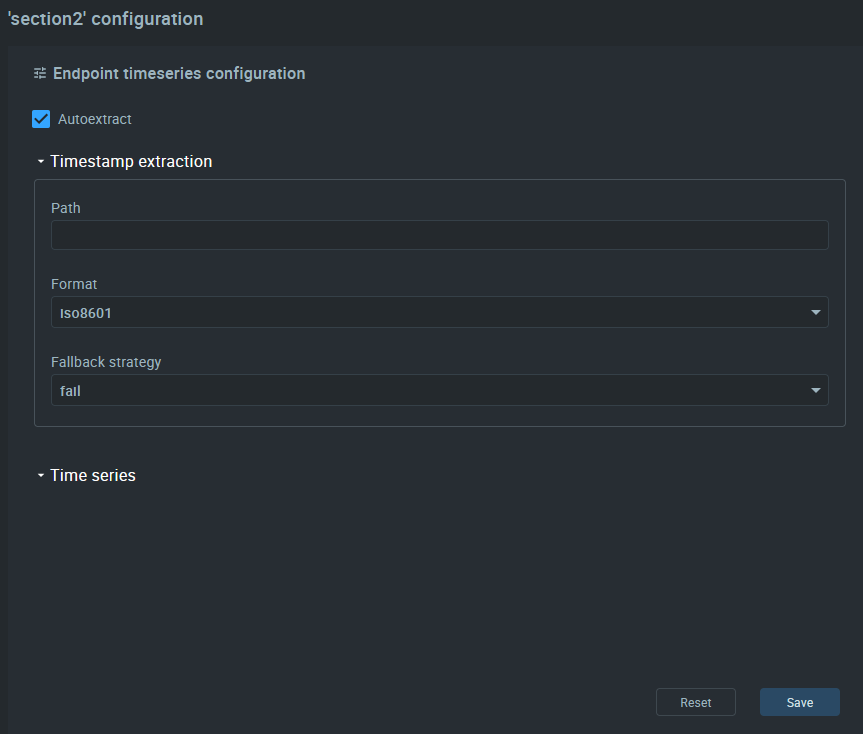
\includegraphics[width=\linewidth]{imagenes/autoextract-option.png}
    \caption{Habilitar opción de auto extracción de datos}
    \label{fig:figure10}
\end{figure}

En nuestro caso hemos creado una versión nueva de nuestra aplicación llamada ``section2`` para probar esta nueva característica de nuestra aplicación. \\

Con esta función activada, se crearán automáticamente series temporales para cada campo numérico que se encuentre en la raíz de las muestras de datos que el endpoint envié. A continuación, podremos ver estas series temporales en la interfaz de usuario del framework, sin necesidad de realizar ninguna configuración adicional. \\

Ahora en la vista de nuestro dispositivo, concretamente en la sección de ``telemetría del dispositivo``, podremos analizar los datos que recoge nuestro dispositivo.

\paragraph{Envio de datos mediante HTTP} \hspace{0pt} \\

Es muy similar a como vimos anteriormente en \ref{http-connection}.

\begin{lstlisting}[language=bash]
curl - -location - -request POST 'https://connect.cloud.kaaiot.com:443/kp1/
<app-version-name>/dcx/<endpoint-token>/json' \
- -data-raw '{
      "intensidad": 50,
      "color": 48
}'
\end{lstlisting}



\paragraph{Envio de datos mediante MQTT} \hspace{0pt} \\

Al igual que en la sección \ref{mqtt-connection} tenemos un código para hacer el envió de datos. En este caso se excluye la carga de configuración y paquetes importados.

\begin{lstlisting}[language=Python]
class DataCollectionClient:

    def __init__(self, client):
        self.client = client
        self.data_collection_topic = f'kp1/{APPLICATION_VERSION}/dcx/{ENDPOINT_TOKEN}/json'

    def connect_to_server(self):
        print(f'Connecting to Kaa server at {KPC_HOST}:{KPC_PORT} using application version {APPLICATION_VERSION} and endpoint token {ENDPOINT_TOKEN}')
        self.client.connect(KPC_HOST, KPC_PORT, 60)
        print('Successfully connected')

    def disconnect_from_server(self):
        print(f'Disconnecting from Kaa server at {KPC_HOST}:{KPC_PORT}...')
        self.client.loop_stop()
        self.client.disconnect()
        print('Successfully disconnected')

    def compose_data_sample(self):
        return json.dumps({
            'timestamp': int(round(time.time() * 1000)),
            'intensidad': random.randint(15, 25),
            'color': random.randint(35, 60),
        })


def on_message(client, userdata, message):
    print(f'<-- Received message on topic "{message.topic}":\n{str(message.payload.decode("utf-8"))}')


def main():
    client = mqtt.Client(client_id=''.join(random.choice(string.ascii_uppercase + string.digits) for _ in range(6)))

    data_collection_client = DataCollectionClient(client)
    data_collection_client.connect_to_server()
    client.on_message = on_message

    client.loop_start()

    listener = SignalListener()
    while listener.keepRunning:

        payload = data_collection_client.compose_data_sample()

        result = data_collection_client.client.publish(topic=data_collection_client.data_collection_topic, payload=payload)
        if result.rc != 0:
            print('Server connection lost, attempting to reconnect')
            data_collection_client.connect_to_server()
        else:
            print(f'--> Sent message on topic "{data_collection_client.data_collection_topic}":\n{payload}')

        time.sleep(3)

    data_collection_client.disconnect_from_server()


class SignalListener:
    keepRunning = True

    def __init__(self):
        signal.signal(signal.SIGINT, self.stop)
        signal.signal(signal.SIGTERM, self.stop)

    def stop(self, signum, frame):
        print('Shutting down...')
        self.keepRunning = False


if __name__ == '__main__':
    main()
\end{lstlisting}

Con este código se entra en un bucle donde se van haciendo llamadas al dispositivo y recogiendo información. La información que nos llega viene en formato JSON que se especifica en la función \textit{compose\_data\_sample}.


\section{Envío de comandos al dispositivo}

En esta sección se trata de ejecutar comandos en nuestro dispositivo.

\subsection{Términos y conceptos}

\subsubsection{Comando}

Un comando es un mensaje de corta duración enviado a un endpoint. Con los comandos se pueden encender y apagar las luces o solicitar un informe inmediato del estado de un endpoint.\\

Cualquier comando puede estar en estado pendiente o ejecutado. El estado pendiente significa que el comando ha sido invocado pero aún no se conoce el resultado de su ejecución. El estado ejecutado se asigna al comando que ha obtenido una respuesta del endpoint, lo que significa que un endpoint recibió el comando, lo ejecutó y envió el resultado de la ejecución a la aplicación.\\

\subsubsection{Tipo de comando}

Representa el comando que se desea ejecutar en un endpoint, por ejemplo, reiniciar o encender la luz. Un endpoint puede manejar tantos tipos de comandos como se definan en su firmware.

\subsection{Pasos a seguir}

\subsubsection{Invocar un comando}

\paragraph{Ejecución con HTTP}  \hspace{0pt} \\

Cuando se invoca un comando en un dispositivo que se conecta a la aplicación a través de un protocolo \textbf{síncrono}, por ejemplo, HTTP, no hay manera de que la plataforma envié dicho comando al dispositivo. En su lugar, el framework persiste el comando y espera hasta que el dispositivo lo solicite para su ejecución. Esto significa que para los dispositivos con protocolos \textbf{síncronos} es nuestra responsabilidad sondear periódicamente la aplicación para nuevos comandos. \\

Para invocar un comando en la sección de ``Dispositivos`` hay un cuadro llamado \textit{Ejecución de comandos}. Aquí indicamos el nombre del tipo de comando y una retención máxima. La retención máxima para la entrega define el tiempo en el que el comando está disponible para su ejecución. Una vez rellenado estos campos podemos clickar en ``run``. Con esto hemos conseguido que si durante la próxima hora se llama a este comando, se ejecutará en el dispositivo. Para hacer la llamada se puede hacer se la siguiente manera:

\begin{lstlisting}[language=bash]
curl --location --request POST 'https://connect.cloud.kaaiot.com:443/kp1/<app-version-name>/cex/<endpoint-token>/command/<command-name>' \
--data-raw '{}'
\end{lstlisting}

Ejecutándolo, obtendremos como respuesta un ID para identificar de forma única el comando. Con la anterior orden hemos conseguido dejar en \textit{Pendiente}. Para ejecutar el comando, mandaremos la siguiente orden:

\begin{lstlisting}[language=bash]
curl --location --request POST 'https://connect.cloud.kaaiot.com:443/kp1/<app-version-name>/cex/<endpoint-token>/result/<command-name>' \
--data-raw '[{
    "id": <command-ID>,
    "statusCode": 200,
    "reasonPhrase": "OK",
    "payload": "Success"
}]'
\end{lstlisting}

Cuando recibe la aplicación el resultado de la ejecución del comando con el ID, marca este como \textit{Ejecutado}.

\paragraph{Ejecución con MQTT}  \hspace{0pt} \\

Con este protocolo el proceso se simplifica. Simplemente tenemos que dejar ejecutando el siguiente código y desde nuestro framework indicamos el tipo de comando y acción sobre el dispositivo.

\begin{lstlisting}[language=Python]
class DataCollectionClient:

    def __init__(self, client):
        self.client = client
        self.data_collection_topic = f'kp1/{APPLICATION_VERSION}/dcx/{ENDPOINT_TOKEN}/json/32'

        command_reboot_topic = f'kp1/{APPLICATION_VERSION}/cex/{ENDPOINT_TOKEN}/command/reboot/status'
        self.client.message_callback_add(command_reboot_topic, self.handle_reboot_command)
        self.command_reboot_result_topik = f'kp1/{APPLICATION_VERSION}/cex/{ENDPOINT_TOKEN}/result/reboot'

        command_zero_topic = f'kp1/{APPLICATION_VERSION}/cex/{ENDPOINT_TOKEN}/command/zero/status'
        self.client.message_callback_add(command_zero_topic, self.handle_zero_command)
        self.command_zero_result_topik = f'kp1/{APPLICATION_VERSION}/cex/{ENDPOINT_TOKEN}/result/zero'

    def connect_to_server(self):
        print(f'Connecting to Kaa server at {KPC_HOST}:{KPC_PORT} using application version {APPLICATION_VERSION} and endpoint token {ENDPOINT_TOKEN}')
        self.client.connect(KPC_HOST, KPC_PORT, 60)
        print('Successfully connected')

    def disconnect_from_server(self):
        print(f'Disconnecting from Kaa server at {KPC_HOST}:{KPC_PORT}...')
        self.client.loop_stop()
        self.client.disconnect()
        print('Successfully disconnected')

    def handle_reboot_command(self, client, userdata, message):
        print(f'<--- Received "reboot" command on topic {message.topic} \nRebooting...')
        command_result = self.compose_command_result_payload(message)
        print(f'command result {command_result}')
        client.publish(topic=self.command_reboot_result_topik, payload=command_result)
        # With below approach we don't receive the command confirmation on the server side.
        # self.client.disconnect()
        # time.sleep(5)  # Simulate the reboot
        # self.connect_to_server()

    def handle_zero_command(self, client, userdata, message):
        print(f'<--- Received "zero" command on topic {message.topic} \nSending zero values...')
        command_result = self.compose_command_result_payload(message)
        client.publish(topic=self.data_collection_topic, payload=self.compose_data_sample(0, 0, 0))
        client.publish(topic=self.command_zero_result_topik, payload=command_result)

    def compose_command_result_payload(self, message):
        command_payload = json.loads(str(message.payload.decode("utf-8")))
        print(f'command payload: {command_payload}')
        command_result_list = []
        for command in command_payload:
            commandResult = {"id": command['id'], "statusCode": 200, "reasonPhrase": "OK", "payload": "Success"}
            command_result_list.append(commandResult)
        return json.dumps(
            command_result_list
        )

    def compose_data_sample(self, fuelLevel, minTemp, maxTemp):
        return json.dumps({
            'timestamp': int(round(time.time() * 1000)),
            'fuelLevel': fuelLevel,
            'temperature': random.randint(minTemp, maxTemp),
        })


def on_message(client, userdata, message):
    print(f'Message received: topic {message.topic}\nbody {str(message.payload.decode("utf-8"))}')


def main():
    # Initiate server connection
    client = mqtt.Client(client_id=''.join(random.choice(string.ascii_uppercase + string.digits) for _ in range(6)))

    data_collection_client = DataCollectionClient(client)
    data_collection_client.connect_to_server()

    client.on_message = on_message

    # Start the loop
    client.loop_start()

    fuelLevel, minTemp, maxTemp = 100, 95, 100

    # Send data samples in loop
    listener = SignalListener()
    while listener.keepRunning:

        payload = data_collection_client.compose_data_sample(fuelLevel, minTemp, maxTemp)

        result = data_collection_client.client.publish(topic=data_collection_client.data_collection_topic, payload=payload)
        if result.rc != 0:
            print('Server connection lost, attempting to reconnect')
            data_collection_client.connect_to_server()
        else:
            print(f'--> Sent message on topic "{data_collection_client.data_collection_topic}":\n{payload}')

        time.sleep(3)

        fuelLevel = fuelLevel - 0.3
        if fuelLevel < 1:
            fuelLevel = 100

    data_collection_client.disconnect_from_server()


class SignalListener:
    keepRunning = True

    def __init__(self):
        signal.signal(signal.SIGINT, self.stop)
        signal.signal(signal.SIGTERM, self.stop)

    def stop(self, signum, frame):
        print('Shutting down...')
        self.keepRunning = False


if __name__ == '__main__':
    main()
\end{lstlisting}

}